\section{The Scyllarus and MIFD systems}
\label{sec:mifd}

Our original system Scyllarus
%% TODO Restore for QR'15
% was an open system which 
performed IDS
fusion on a diverse set of third party \idses~\anoncite{goldman:discex2001,goldman:discex2001}.
Its successor,
MIFD (Model-based Intrusion Fusion and Detection),
enhances Scyllarus
%% TODO Restore for QR'15
% as part of the STRATUS system's integration of
 to integrate
IDS fusion into a comprehensive suite for cyber defense
\anoncite{thayer13:_compar_strat_tactic_respon_cyber_threat}.
For simplicity we refer to our \ids fusion system as ``MIFD,'' but
except where we specify otherwise, our account applies to Scyllarus as well.

The first tasks performed by MIFD are
\emph{collection} and \emph{translation}: IDS reports
must be collected and presented to MIFD, and
must be translated into a common
sensor report data structure for processing.
We will not discuss these less interesting
preliminaries, except to mention that they
involve a substantial amount of data rectification
%% TODO Restore for QR'15
 to address the lack of standardization in data formats and event taxonomies.
%.  There is no widely-accepted
%common data format (the proposed IDMEF standard~\cite{IDMEF} has not caught on), nor
%is there an accepted taxonomy for events or event roles (e.g., the widely used ``source''
%and ``destination'' are not consistently applied).
%These problems are exacerbated by the fact that intrusion detection ``systems''
%are often simply a casually-assembled anthology of rules by different authors running in the same
%framework.

{\ids} fusion proper begins with
\textbf{Clustering.} From the
sensor reports,
and based on an ontology detailing how (and with what probability)
sensor reports may correspond to events,
MIFD generates \emph{event hypotheses} to represent the
underlying events of interest that may have caused the sensor reports.  A
sensor report that provides evidence for an event hypothesis is a
\emph{supporter}.
The clustering process constructs a
directed graph of event hypothesis and sensor report nodes forming a
Bayesian belief network.

Figure \ref{fig:bnets}(a) shows the Bayes net generated by MIFD for
the very simple case of a single event hypothesized to be the cause of
a number of sensor reports.  In general sensor reports will be
ambiguous, each supporting several different event hypotheses.
Figure~\ref{fig:bnets}(b) shows a more complex example where sensor reports
might be caused by two different underlying events.
Finally, Figure~\ref{fig:bnets}(c) shows a more complex example where an event
has two component sub-events.
%% DONE: cut the following sentence because its meaning wasn't
%% clear.... I think what's meant is something like "label" rather than
%% "measurement," but I couldn't figure out how to clarify it. --- How
%% about this?
% The sensors themselves are simply either on or off, without any additional
% outputs which would distinguish hypotheses.

\ids rules detect indirect features of intrusions, but they typically
report only the intrusion that their designer believes has caused the feature.
This creates a number of problems, first and foremost that the
sensors have high false positive rates.
For example, a local software update server
may look like an attacker performing reconnaissance.
Worse, some false positives are correlated: the normal
activity of a print server may be mis-detected as a scan by several
different sensors.
To handle simple sensor failures, MIFD associates with each sensor a false
positive likelihood.
But to address the correlated false positives such as the scanning example, we
introduce benign events, that can compete with attack and (simple) false
positive explanations for results.\footnote{Where possible, we try to introduce sensors that
can specifically detect the benign events. 
%% TODO Restore for QR'15
%To return to our earlier example, we
%might introduce a ``print server sensor'' to help disambiguate detections. We do
%not address this issue in our experiments.
}
% FIXME: Add a figure 2(c) -- or separately numbered figure -- where we have a
% benign event, explaining two of the sensor reports, as well as the two attack
% events. 
Another problem with indirect sensing is that the sensors are often imprecise:
the features that they detect often occur not only in the absence of the
advertised intrusion, but in the presence of \emph{other} intrusions with
similar characteristics.

%% TODO Restore for QR'15 --- we'd earlier discussed
%% removing this paragraph anyway.
%MIFD also has \emph{complex} events that have component sub-events, such as a
%phishing attack with component events phishing email and drive-by-download.
%Our current experiments do not address the role of complex events, so we will
%not discuss them further.

\begin{figure}
  \centering
  \begin{tabular}{c@{\hspace{1cm}}c}
  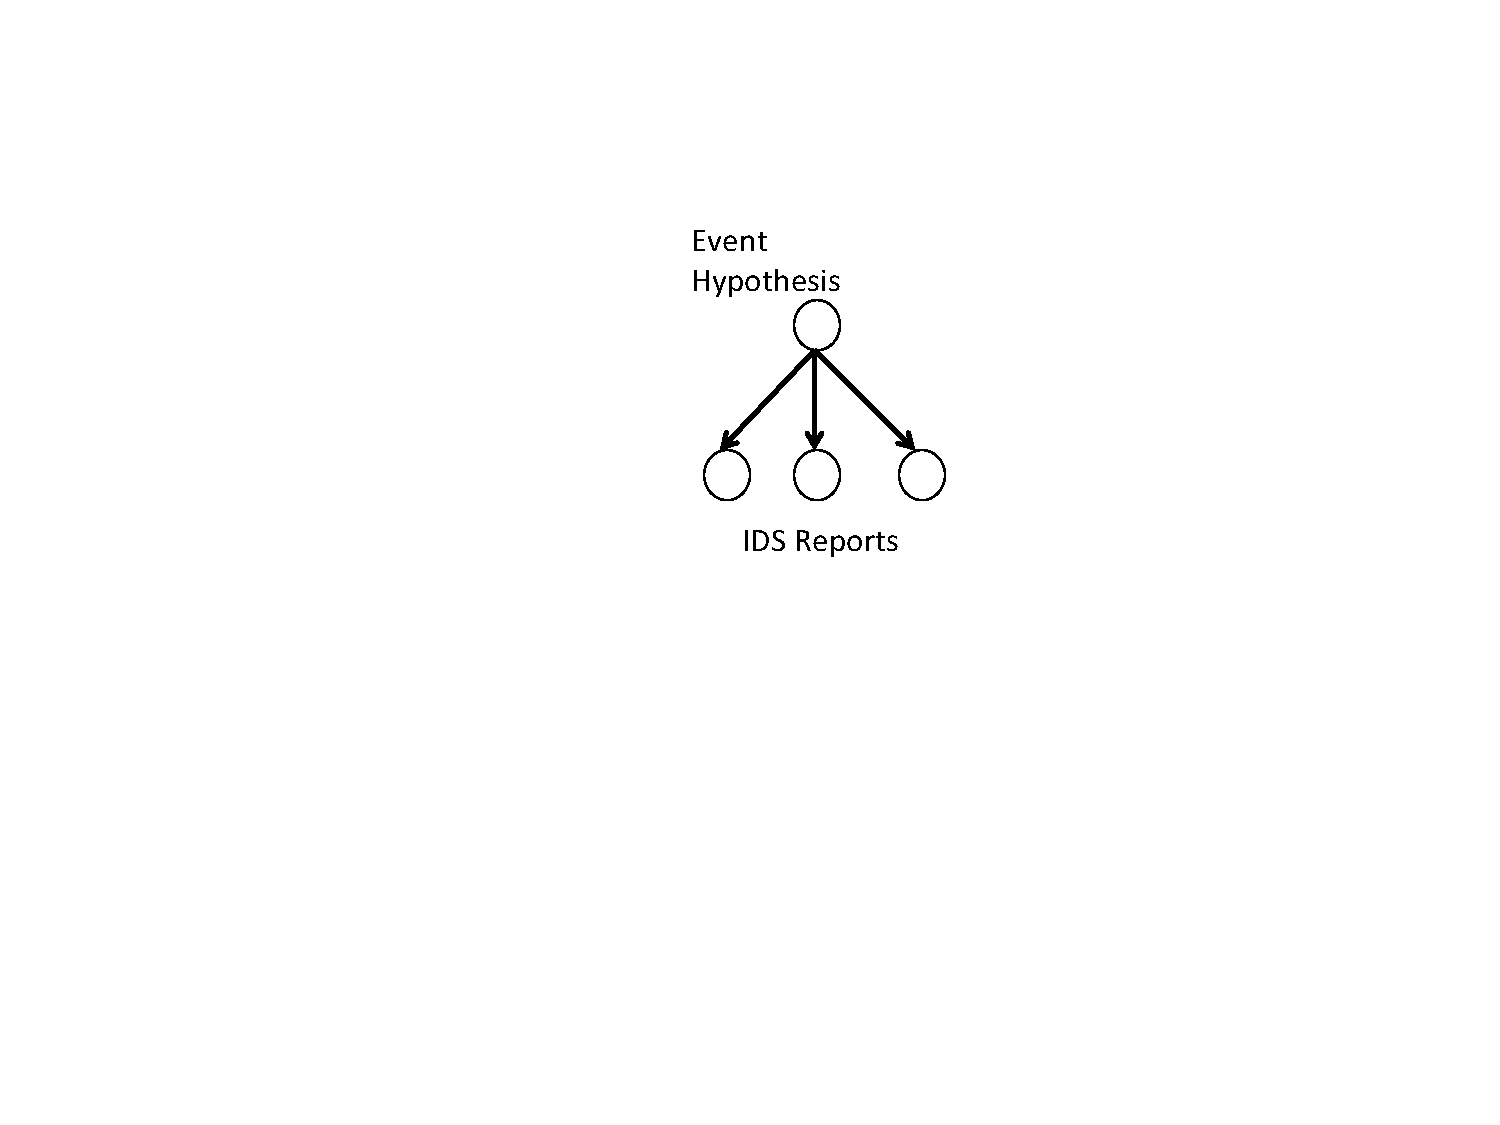
\includegraphics[width=.2\columnwidth]{figures/bnets1-cropped.pdf} &
  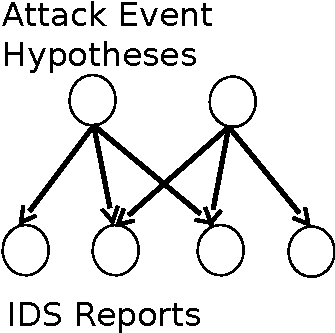
\includegraphics[width=.267\columnwidth]{figures/bnets2-cropped.pdf} 
  \\ (a) & (b) \\
  \end{tabular}
  \newline{}
  \begin{tabular}{c}
  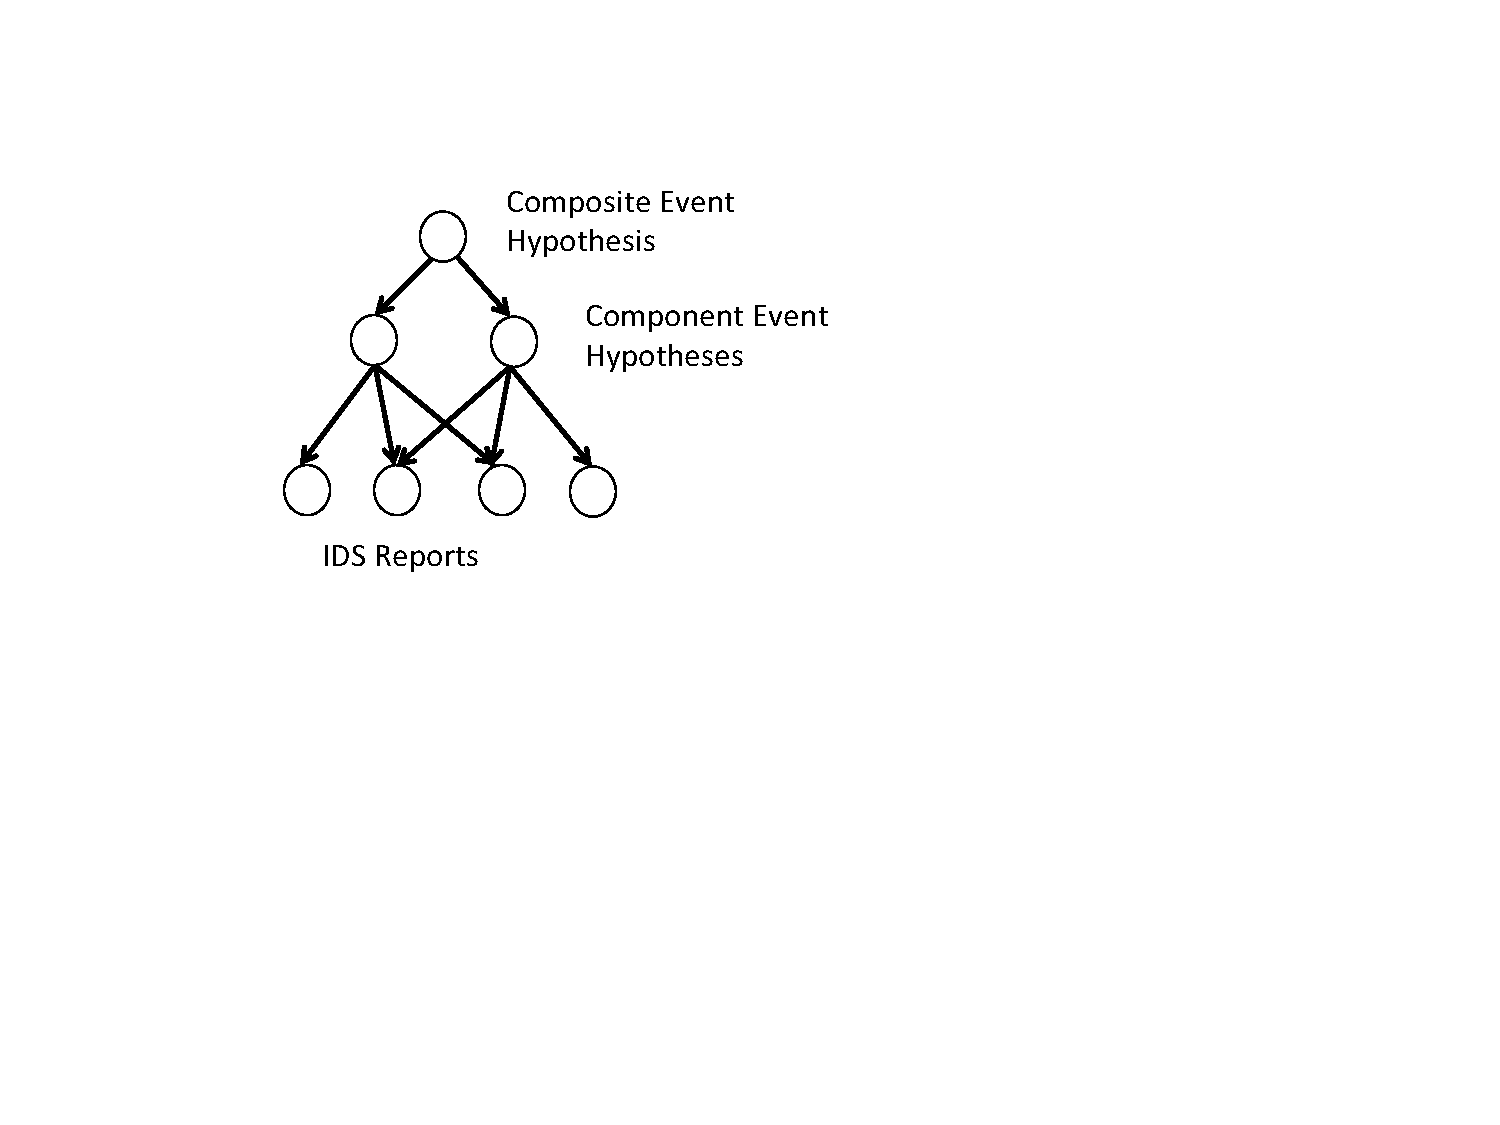
\includegraphics[width=.4\columnwidth]{figures/bnets3-cropped.pdf} 
    \\ (c)
  \end{tabular}
  \caption{Bayes networks generated by MIFD.}
  \label{fig:bnets}
  
\end{figure}

The second inference step is \textbf{Assessment,} in which MIFD assigns a degree of belief
to each of the event hypotheses.
MIFD does this by performing Bayesian updating on the belief network constructed
by the clustering process. 
%% As we discuss below, MIFD does this using the \zplus qualitative probability
%% scheme rather than standard probability theory.
%%

Note that Scyllarus and MIFD are intended as long-running online services, not batch processes.
Scyllarus has run for months at a time.
One major requirement for such long-term operation is that the
inference steps must be performed cyclically.  MIFD repeatedly reads
reports and clusters them, periodically interrupting that
cycle to perform assessment.
Scyllarus also periodically flushes older events and reports out of working
memory (they persist in a database).

%% FIXED Although this next sentence is a true fact, I'm not sure it
%% belongs here --- it makes assessment efficient, but that's not per
%% se an inherent requirement for long-term operation.
% Moreover, in general the Bayesian belief network
% is not fully connected, so for efficiency MIFD assesses each connected
% component individually.
% \footnote{%
%   An additional essential requirement for long-term operation, not
%   relevant to the remainder of this presentation, is some form of
%   garbage collection: old event hypotheses and sensor reports
%   guaranteed no longer to be relevant to subsequent report must be
%   removed from working memory.}

% \subsection{System Z+}
% \label{sec:zplus}

MIFD
follows Pearl's exhortation~\shortcite{Pearlbook} that the core of probability theory is
the patterns of inference it enables (explaining away, combining forward causal
inference and evidential reasoning, etc.), rather than precise numerical
calculations.  He recommends these patterns be used even when precise numbers are
not available.
%% TODO Restore for QR'15
%As outlined above,
MIFD treats
\ids fusion as an abductive problem, formalized using Bayes nets.
But precise values for the parameters of these Bayes nets
%% TODO Restore for QR'15
% --- probabilities of attacks, false positives, false negatives, etc. ---
are \emph{never} available to us: populations of
attacks and attackers change, different networks have little in common with each other, distributions are
non-stationary, etc.  Moreover these difficulties are not solvable via machine learning:
Sommer and Paxson~\shortcite{Sommer10outsidethe} discuss the challenges \idses pose to ML.

Goldszmidt and
Pearl's \zplus{}~\shortcite{Goldszmidt:96}
shares the
basic structure of normal probability theory but abstracts the actual
probabilities.
Events have a natural number rank \tkappa{}
corresponding to their degree of surprise (so a rank of one is more surprising
than zero). The semantics of this scheme comes from a set of probability
distributions in which the probabilities are polynomials over some infinitesimal
$\epsilon$. In this scheme, the \tkappa{} corresponds to the exponent
of the polynomial's leading term.
%% TODO Restore for QR'15
%As we mentioned earlier, 
\zplus is similar to the ``big-$O$'' method used
in analysis of algorithms.
With this semantics \zplus{}
provides a ``ladder'' of events of qualitatively different
orders of likelihood.
%% TODO Restore for QR'15
%Note that \zplus is very different from Wellman's qualitative probability
%networks~\cite{Wellman:90}, whose abstraction is based on direction of change, rather than order
%of magnitude relations ``at rest,'' as it were.
%Wellman's approach is more relevant when choosing interventions (as in his work
%on medical diagnosis and treatment), and less for fusion.

\hide{
The \assessor{} must combine the judgments of a wide variety of intrusion
detection systems (and potentially other relevant information sources), that use
widely varying sources of information and algorithms. Further, in general we
will not have access to the internals of these sensors.  In such an environment,
it is not realistic to expect good models of the response of these sensors; in
particular, exact measures of P(sensor response|event) are not available.  There
have been some attempts to investigate sensor response (e.g., the studies
conducted by Lincoln Labs~\cite{lippmann00:eval}), but the results seem heavily dependent on the
context in which the sensors are deployed.

The issue of prior probabilities also militates against the use of exact
probabilities.  In order to use an exact Bayesian method, we would need not only
the detection probability, $P(\mathit{sensor\ response}|\mathit{event})$, and
the false alarm probability, $P(\mathit{sensor\ response}|\neg \mathit{event})$,
but also $P(\mathit{event})$, a measure of the prior
probabilities of the events that interest us, in this case the attacks and the
benign events that can cause false positives.  Even in the most constrained
environments, the probabilities of the various attacks, are unlikely to be
available to us,  and the Scyllarus system is designed for application across a
wide variety of enterprises.  Further, the probability distributions for benign
events are likely to be of odd forms (e.g., one's own network-mapping software
runs at particular times of the day).  So our solution must tolerate vague
measures of likelihood.

Finally, in this domain, as with most practical applications of probabilistic
updating, the effect of the evidence will \emph{usually} overwhelm the effect of the prior
likelihoods(e.g., \cite{pradhan:96}). So inexactitude in the quantities specified will not matter to our
final conclusions.}

Under \zplus\ we may apply the normal operation
of probability theory
%% TODO Restore for QR'15
% --- conditionalization, Bayes' law, etc. ---
but the arithmetic operations we use for them change.  Rather than multiplying
probabilities, we add degrees of surprise%
%% TODO Restore for QR'15, but it's in the table anyway
%; rather than adding
%probabilities, we take the minimum surprise%
.  Goldszmidt and
Pearl~\shortcite{Goldszmidt:96} provide the following substitutions
between the quantitative probability function $P$ and its qualitative
counterpart $\kappa$ for formulas $\phi$ and $\psi$, and primitive events, $e$.
\begin{displaymath}
  \small
  \begin{array}{|l|l|}
    \hline
  P(\psi) = \sum_{e \in \psi} P(e) & \kappa(\psi) =
  \operatorname{min}_{e \in \psi} \kappa(\phi) \\ \hline
  P(\psi) + P(\neg \psi) = 1 & \kappa(\psi) = 0 \vee \kappa(\neg \psi) = 0
  \\ \hline
  P(\psi | \phi) = P(\psi \wedge \phi) / P(\phi) &
  \kappa(\psi | \phi) = \kappa(\psi \wedge \phi) - \kappa(\phi)
  \\ \hline
\end{array}
\end{displaymath}
\noindent
In a Bayes network, with conditionally independent $\omega$ and
$\phi$ we further have $\kappa(\omega \wedge \phi) = \kappa(\omega) + \kappa(\phi)$.
\hide{Instead of the probability
of an event being the sum of the probabilities of the primitive outcomes that
make up that event, the degree of surprise of an event is the minimum of the
degrees of surprise of the primitive outcomes that make it up. Instead of having
the probabilities of mutually exclusive and exhaustive events sum to one, at
least one of a set of mutually exclusive and exhaustive events must be
unsurprising. Finally, we have an analog of Bayes' law in which the normalizing
operation consists of subtraction rather than division.
}

\hide{We used Bayesian networks to help us in modeling and solving the correlation problem. Bayesian networks are 
ways of graphically capturing probabilistic reasoning. They are useful in expert systems because they 
simplify knowledge acquisition and, by capturing (conditional) independences, simplify computation 
(Pearl, 1988). In particular, in the domain of intrusion detection, Bayes nets help us capture several 
important patterns or probabilistic reasoning:
\begin{itemize}
\item	Reasoning based on evidence merging; 
\item	``Explaining away'' reports by alternative explanations.  E.g., if a benign event accounts for a number 
of reports, those reports will be explained away, and no longer provide support for more alarming 
hypotheses.

\item	Abstraction reasoning that employs the sub\-class/su\-per\-class relationships in the event dictionary.

\item	Part/whole reasoning, to recognize complex composite events.

\item	Distinguishing between judgments that are based on different sensor bases and those that use the same 
sensor.  This helps us distinguish between cases when two sensors provide support for each other and 
when we simply have redundant reports (e.g., two network intrusion detection systems using exactly 
the same algorithm that see the same traffic, at two different points).
\end{itemize}
A Bayesian network is a directed, acyclic graph (DAG) depicting a set of random variables. Edges between 
nodes in the DAG represent causal influences. Using a Bayesian network, we can capture a joint 
distribution factorized into unconditional probabilities for root nodes and conditional probability tables for 
non-root nodes. The conditional probability tables contain probability distributions for the child nodes, 
conditioned on all the values of their parents.
}

There are a number of efficient algorithms for finding the posterior distributions of Bayesian networks, 
conditional on observations of some of the random variables. These algorithms may readily be adapted to 
provide posterior $\kappa$ rankings instead of probabilities.
MIFD translates Bayes networks into an
%% DONE Charniak:88 is Charniak and Goldman --- withhold this one too? No --
%% it's not obviously tied to this paper, so we don't need to worry about it
%% breaching anonymity. [2014/08/24:rpg]
ATMS~\cite{Forbus+DeKleer:1993}; see
%% For anonymous:
%\cite{Charniak:88,Poole:93,provan-ijcai89}
%and \anoncite{goldman:09Scyllarus}
%% De-anonymized:
\cite{Charniak:88,Poole:93,provan-ijcai89,goldman:09Scyllarus}
%
for this encoding.
This implementation is not especially efficient, but we have found
it is I/O which dominates runtime, and we apply several optimizations to
handle common special cases.
%% TODO Restore for QR'15
%To date (somewhat to our disappointment!) optimizing the general \zplus
%inference method has not been key to system performance.
%
% To date, finding the optimal inference method
% % in terms of runtime
% has been
% less important than finding an algorithm easy to modify for \zplus.

MIFD's assessment ranks hypotheses as either
\emph{likely}, \emph{plausible} or \emph{unlikely}. A hypothesis $h$,
conditioned on evidence $\omega$,
is \emph{likely} if
$\kappa(h|\omega) < \kappa(\neg h|\omega)$, \emph{plausible} if $\kappa(h|\omega) = \kappa(\neg h|\omega)$
and \emph{unlikely} otherwise.

The MIFD system requires comparatively few \tkappa parameters given the above
design.  For sensors, we need \fpKappa, and for events (attack and benign)
we need $\kappa(\text{event})$.  In practice, we assign global defaults for
these, based on how generally accurate the input \idses are: for example, we set
these \tkappa\ values so that it takes $n = 2\ \text{or}\ 3$ sensors for us to judge an event
as \emph{likely}, with
the following consistency constraints:
\begin{align}
  \label{eqn:coherence-ineq}
  \kappa(\text{false-positive}),\kappa(\text{benign})
  &< \kappa(\text{attack}) \\
 &< n \cdot \kappa(\text{false-positive}) \nonumber
\end{align}
That is, a single sensor false positive is less surprising than an
  attack event;
a benign event is also less surprising than an attack; and
an attack is less surprising than false positives from $n$
  of the sensors detecting that event.
%
With a few exceptions, this paper assumes $n=3$ sensors, so we
have $0 < \kappa(\text{benign}) < \kappa(\text{attack}) 
    < 3 \kappa(\text{false-positive})$.
% \begin{displaymath}
%   \begin{split}
%     0 &< \kappa(\text{benign-event}) < \kappa(\text{attack-event}) \\
%     &< 3 \kappa(\text{false-positive})
%   \end{split}
% \end{displaymath}
% \noindent
In actual deployments, we then
nudge the false positive rankings up in the rare cases where we have a
particularly good sensor, or down if we have a particularly bad sensor.
%% TODO Restore for QR'15
%We are less likely to adjust attack event probabilities, but
%there are exceptions such as scanning (very common), and some complex events.


%%% Local Variables: 
%%% mode: latex
%%% TeX-master: "main"
%%% End: 


% Not sure that the reader cares about the data model, yet.  Maybe; maybe not.
\hide{%
\mifd\ operates under the following data model:  It receives
\emph{sensor reports} and generates \emph{event
  hypotheses}. Hypotheses include a \emph{likelihood} slot, which
\mifd\ may update as it receives additional reports, plus a list of
\emph{supporters} which may be either sensor reports or other
hypotheses. Both sensor reports and hypotheses have a list of
\emph{supports}, inverse to the \emph{supporters} relationship.
Both reports and hypotheses are associated with \emph{prototype}
objects which contain information common to all instances sharing a
prototype. In particular:
\begin{compactitem}
\item Sensor report prototypes include a slot for the (natural
  number-valued) qualitative probability of false positives for the
  report.
\item Event prototypes include a slot for the qualitative
  probability of the event occurring.
\end{compactitem}
The relationship between reports and events is modeled to \mifd\ as
\emph{hypothesis matchers}, which pair a report prototype and an event
prototype. Each instance where a particular sort of event might
trigger a particular sort of report is modeled as a separate
hypothesis matcher, so there may be several hypothesis matchers
pertaining to each sensor report prototype.  In an initializing step,
\mifd\ creates a table of hypothesis matchers indexed by sensor report
prototypes.

\mifd\ provides two operations, \emph{clustering} and
\emph{assessing}.  Clustering occurs whenever \mifd\ receives a new
sensor report.  For each of the event prototypes paired with the new
report's prototype by some hypothesis matcher,
\begin{compactitem}
\item If there are existing hypotheses with that event prototype, then
  \mifd\ adds the new report as a supporter of these hypotheses.
\item If there are no existing hypotheses with that event prototype,
  then \mifd\ creates a new hypothesis with the new report as its sole
  supporter.
\end{compactitem}

Assessment occurs whenever \mifd\ is required to produce updates to
hypothesis likelihood. Each sensor report could individually justify
possibly many events, but in assessment \mifd\ distinguishes more
likely hypothesized events from less likely ones, taking into account
all reports and the prior probabilities of hypothesized events and
report false positives.  We can first decompose this task by
considering the graph formed by the \emph{supporters} relationship on
reports and hypotheses, and consider the connected subgraphs in
turn. Moreover, we need consider only those subgraphs containing a
sensor report received since the last assessment.

To distinguish the more and less likely hypothesized events in each
connected subgraph, \mifd\ uses an assumption-based truth maintenance
system (ATMS). An ATMS is a directed, acyclic hypergraph in which
nodes represent possibly-true statements, and hyperedges from $N$
nodes to a single node represent an inference from the $N$ statements
concluding the single statement~\cite{Forbus+DeKleer:1993}. The
initial nodes of the ATMS hypergraph are called \emph{assumptions}; in
\mifd's use of ATMSs there are three forms of assumption:
\begin{compactitem}
\item ``Event $X$ did happen.''
\item ``Event $Y$ did not happen.''
\item ``Sensor report $Z$ was a false positive.''
\end{compactitem}
Corresponding pairs of the first two forms are marked in the ATMS as
\emph{nogood}.  Node representing that an event occurred can be
justified either the corresponding event assumption, or by other
events which can be generalized or collected together; nodes
representing the receipt of a sensor report can be justified either by
an event's node, or by a false positive and the negation of an event
happening.

As an ATMS's hypergraph is constructed, the ATMS algorithm maintains
the list of minimal consistent assumption sets that justify each node.
\mifd\ is interested in the most likely consistent assumption sets
satisfying the sensor report nodes, that is, those which have the
lowest total qualitative probability rank.  In principal \mifd\ could
simply add another ``goal'' node justified by the sensor report nodes,
use the ATMS algorithm to maintain its assumption sets, and find the
most likely ones. But in practice this is not a feasible approach;
finding all such consistent sets simply overwhelms the ATMS algorithm.
Instead \mifd\ performs an A* search to find the most likely unions of
assumption sets from each of the sensor node labels.

Finally, to determine the likelihood of each hypothesized event $E$,
\mifd\ looks for the presence of the assumptions that $E$ did or did
not happen in the most likely assumption sets. If only the positive
assumption occurs in these sets, then the hypothesis is deemed
\emph{likely}, the highest of the three output qualitative probability
values; if only the negative assumption occurs, then \emph{unlikely},
the lowest. If both positive and negative assumptions occur, then the
hypothesis is given a third, middle value \emph{plausible}.}

% Because the domain does not afford us access to good statistics, we do not use
% conventional Bayesian reasoning.  Instead, we use a qualitative abstraction of
% probabilistic reasoning, very similar to the big-O scheme familiar to computer
% scientists, \emph{\zplus}~\cite{Goldszmidt:92,Goldszmidt:92a,Goldszmidt:96}.


%%% Local Variables: 
%%% mode: latex
%%% TeX-master: "main"
%%% End: 
